\chapter{Đường cong Lợi suất Trái phiếu Chính phủ}
\label{ch:M1L3}

\section*{Lesson Notes}

\textbf{Dự án} \\
\textbf{Thời gian đọc:} 60 phút \\
\textbf{Kiến thức nền tảng:} Trái phiếu Kho bạc Hoa Kỳ (U.S. Treasury Bonds), Đường cong lợi suất (Yield Curve), Đại số tuyến tính (Linear Algebra), Python cơ bản \\
\textbf{Từ khóa:} Đường cong giá-lợi suất trái phiếu (Bond price-yield curve), Lãi suất phi rủi ro (Risk free interest rate), Nelson Siegel, Spline bậc ba (Cubic Spline)

Trong bài học trước, chúng ta đã tìm hiểu cách lấy thông tin về lợi suất Trái phiếu Kho bạc Hoa Kỳ và đi qua một số khái niệm nền tảng về đường cong lợi suất. Trong bài học này, chúng ta sẽ đi sâu hơn và tìm hiểu cách khớp (fit) một đường cong lợi suất trái phiếu. Chúng ta sẽ tiếp tục sử dụng dữ liệu lợi suất Trái phiếu Kho bạc Hoa Kỳ để làm ví dụ minh họa.

\section[Lãi suất Phi rủi ro]{Lãi suất Phi rủi ro (Risk-Free Interest Rates)}

Trong khóa học Thị trường Tài chính, chúng ta đã tìm hiểu về rủi ro tín dụng khi đầu tư vào trái phiếu. Rủi ro tín dụng, được gánh chịu bởi nhà đầu tư trái phiếu, là rủi ro mà tổ chức phát hành trái phiếu sẽ vỡ nợ (default). Một thực thể có xếp hạng tín dụng hoặc điểm tín dụng cao có thể vay tiền từ các thị trường tài chính với mức lãi suất thấp hơn so với một thực thể có xếp hạng tín dụng thấp hơn. Tại Hoa Kỳ, các trái phiếu do chính phủ phát hành (Trái phiếu Kho bạc Hoa Kỳ hay Treasuries) thường được coi là trái phiếu có xếp hạng tín dụng cao. Do đó, lợi suất Trái phiếu Kho bạc thường được sử dụng làm lãi suất phi rủi ro cho việc định giá trái phiếu trong ngành tài chính. Có rất nhiều cuộc tranh luận về việc liệu Trái phiếu Kho bạc Hoa Kỳ có thực sự an toàn với rủi ro vỡ nợ bằng không hay không. Những kịch bản khác nhau sẽ cần những cân nhắc khác nhau. Trong bài học này, chúng ta sẽ tuân theo quy ước hiện hành của thị trường tài chính bằng cách sử dụng lợi suất Trái phiếu Kho bạc Hoa Kỳ làm lãi suất phi rủi ro.

Một khái niệm quan trọng khác trong rủi ro tín dụng là phần bù rủi ro tín dụng (credit spread). Chênh lệch tín dụng hay phần bù tín dụng là khoảng chênh lệch lãi suất giữa một trái phiếu doanh nghiệp và một trái phiếu chính phủ có cùng kỳ hạn. Khoảng chênh lệch lãi suất này cũng được gọi là lợi suất vượt trội (excess return) của trái phiếu doanh nghiệp vì lợi suất trái phiếu chính phủ là lãi suất phi rủi ro. Lợi suất vượt trội của trái phiếu doanh nghiệp là phần lợi nhuận tăng thêm dành cho người nắm giữ trái phiếu doanh nghiệp để họ chấp nhận gánh chịu rủi ro bổ sung khi nắm giữ trái phiếu này.

Vì lãi suất phi rủi ro là một yếu tố then chốt không chỉ trong định giá trái phiếu mà còn trong định giá các tài sản tài chính khác và quản lý danh mục đầu tư, nên việc hiểu được các đặc điểm và hành vi của lãi suất phi rủi ro là vô cùng quan trọng. Trong bài học này, chúng ta sẽ sử dụng lợi suất trái phiếu (hay các trái phiếu) kho bạc Hoa Kỳ làm lãi suất phi rủi ro để điều tra hành vi của chúng và tiến hành phân tích.

\section[Biến động của Lợi suất Trái phiếu Kho bạc Hoa Kỳ]{Biến động của Lợi suất Trái phiếu Kho bạc Hoa Kỳ (Volatility of U.S. Treasury Yields)}

Đầu tiên, hãy xem xét các mức độ biến động của lợi suất Trái phiếu Kho bạc ở các kỳ hạn khác nhau. Chúng ta tiếp tục phương pháp của Bài 2 để lấy dữ liệu lợi suất Trái phiếu Kho bạc từ FRED bằng Python như sau.

\begin{lstlisting}[language=Python]
In [1]: import pandas as pd
        from fredapi import Fred
        import matplotlib.pyplot as plt
        import seaborn as sns
        sns.set()
\end{lstlisting}

\begin{lstlisting}[language=Python]
In [2]: # Initialize the FRED API with your key
        fred = Fred(api_key='5079f41d061a4037d81f3da69e018803') # Replace my APIKEY
        
        # List of Treasury yield series IDs
        series_ids = ['DGS1MO', 'DGS3MO', 'DGS6MO', 'DGS1', 'DGS2', 'DGS3', 'DGS5',
                      'DGS7', 'DGS10', 'DGS20', 'DGS30']
                      
        # Function to get data for a single series
        def get_yield_data(series_id):
            data = fred.get_series(series_id, observation_start="1975-01-01", observ
            return data
            
        #Get data for all series
        yields_dict = {series_id: get_yield_data(series_id) for series_id in series_
        
        # Combine into a single DataFrame
        yields = pd.DataFrame(yields_dict)
        
        # Rename columns for clarity
        yields.columns = ['1 Month', '3 Month', '6 Month', '1 Year', '2 Year', '3 Ye
                          '7 Year', '10 Year', '20 Year', '30 Year']
\end{lstlisting}

\begin{lstlisting}[language=Python]
In [3]: yields.index = pd.to_datetime(yields.index)
\end{lstlisting}

Bây giờ chúng ta hãy tính độ lệch chuẩn của lợi suất Trái phiếu Kho bạc ở các kỳ hạn khác nhau. Sau đó, chúng ta sẽ vẽ một đồ thị để trình bày các độ lệch chuẩn theo kỳ hạn.

\begin{lstlisting}[language=Python]
In [4]: yields = yields.dropna()
        y_std = yields.std()
        y_std
\end{lstlisting}

\begin{lstlisting}[language=Python]
Out [4]: 1 Month    1.705851
         3 Month    1.733347
         6 Month    1.746829
         1 Year     1.684091
         2 Year     1.545413
         3 Year     1.446639
         5 Year     1.309345
         7 Year     1.226457
         10 Year    1.174092
         20 Year    1.206514
         30 Year    1.108774
         dtype: float64
\end{lstlisting}

\begin{lstlisting}[language=Python]
In [5]: fig, ax = plt.subplots()
        y_std.plot(figsize=(8,5), marker='o', title='Figure 0, Standard Deviations
        plt.xlabel("Maturity")
        plt.ylabel("Standard Deviation")
        
        for i in range(len(y_std)):
            ax.annotate(str(round(y_std.iloc[i], 2)), xy=(i,y_std.iloc[i]))
            
        plt.show()
\end{lstlisting}

\begin{figure}[htbp]
    \centering
    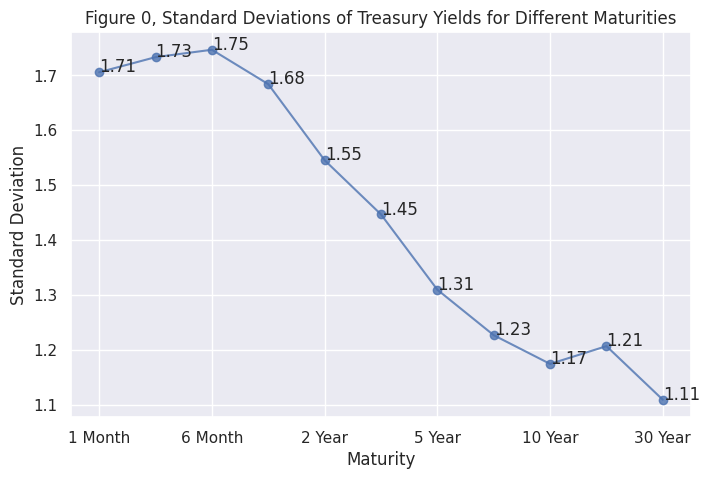
\includegraphics[width=0.8\textwidth]{gfx/m1l3_notes_fig0_std_deviations.png}
    \caption{Hình 0, Độ lệch chuẩn của Lợi suất Trái phiếu Kho bạc theo các Kỳ hạn khác nhau}
    \label{fig:m1l3_fig0}
\end{figure}

Từ đồ thị trên, chúng ta thấy rằng độ lệch chuẩn của trái phiếu Kho bạc Hoa Kỳ có kỳ hạn ngắn cao hơn so với trái phiếu Kho bạc Hoa Kỳ có kỳ hạn dài hơn. Độ lệch chuẩn đối với các trái phiếu Kho bạc có kỳ hạn dưới một năm duy trì ở mức cao trên 1,7. Sau đó, độ lệch chuẩn của các trái phiếu Kho bạc có kỳ hạn trên một năm giảm đều.

\section[Đường cong Giá - Lợi suất Trái phiếu Kho bạc]{Đường cong Giá - Lợi suất Trái phiếu Kho bạc (Treasury Bond Price-Yield Curve)}

Theo công thức toán học về giá trái phiếu, mối quan hệ giữa giá trái phiếu và lợi suất trái phiếu là phi tuyến. Mối quan hệ này được giải thích tốt nhất thông qua đường cong giá - lợi suất trái phiếu. Hãy sử dụng hình sau đây để minh họa mối quan hệ này.

\textbf{Hình 1: Đường cong Giá - Lợi suất Trái phiếu} \\
\textit{Đồ thị thể hiện giá so với lợi suất với một đường thẳng cắt một đường cong tại một điểm được đánh dấu}

Trong Hình 1, chúng ta có thể thấy rằng khi lợi suất/lãi suất của một trái phiếu tăng, giá của trái phiếu sẽ giảm. Ngược lại, khi lợi suất/lãi suất của trái phiếu giảm, giá của trái phiếu sẽ tăng. Có một mối quan hệ nghịch biến giữa giá trái phiếu và lợi suất trái phiếu. Tuy nhiên, khi lợi suất thay đổi một đơn vị, mức độ thay đổi của giá sẽ khác nhau tùy thuộc vào việc mức lợi suất đang ở đâu khi sự thay đổi lợi suất xảy ra.

Đây là một điểm then chốt khác cần chú ý trong mối quan hệ giá - lợi suất trái phiếu: giá trái phiếu và lợi suất trái phiếu không có mối quan hệ tuyến tính; chúng có mối quan hệ lồi (convex). Mối quan hệ phi tuyến giữa giá trái phiếu và lợi suất trái phiếu có ý nghĩa quan trọng trong quản trị rủi ro lãi suất đối với đầu tư trái phiếu. Hãy sử dụng Hình 2 sau đây để giải thích khái niệm này.

\textbf{Hình 2: Mối quan hệ Phi tuyến giữa Giá Trái phiếu và Lợi suất Trái phiếu} \\
\textit{Đồ thị thể hiện giá so với lợi suất với hai hình chữ nhật (D1, D2) minh họa sự thay đổi của giá (P1, P2) dọc theo một đường cong dốc xuống}

Dựa trên tính chất lồi của đường cong giá-lợi suất trái phiếu được mô tả trong Hình 2, mức độ thay đổi giá khi lợi suất thay đổi một lượng như nhau sẽ khác nhau tùy thuộc vào mức lợi suất. Trong Hình 2, D1 và D2 có cùng độ dài. Khi lợi suất thay đổi một khoảng D1, mức độ thay đổi giá là P1. Khi lợi suất thay đổi một khoảng D2, mức độ thay đổi giá là P2. Tuy nhiên, mức lợi suất cho D1 cao hơn mức lợi suất cho D2. Do tính lồi của đường cong giá-lợi suất, P1 nhỏ hơn P2.

Đặc tính này của mối quan hệ giữa giá trái phiếu và lợi suất trái phiếu được gọi là độ cong (curvature). Ví dụ trên chứng minh rằng độ dốc của đường cong giá-lợi suất thay đổi khi mức lợi suất thay đổi. Độ cong của đường cong giá-lợi suất được sử dụng để mô tả sự phụ thuộc của độ dốc này vào mức lợi suất. Một nhà quản lý danh mục đầu tư trái phiếu sẽ phải chú ý đến độ cong của các khoản nắm giữ trái phiếu khi quản trị rủi ro lãi suất.

\section[Khớp Đa thức cho Đường cong Lợi suất Trái phiếu Kho bạc Hoa Kỳ]{Khớp Đa thức cho Đường cong Lợi suất Trái phiếu Kho bạc Hoa Kỳ (Polynomial Fitting for U.S. Treasury Yield Curve)}

Chúng ta đã nói về đường cong lợi suất Trái phiếu Kho bạc Hoa Kỳ trong bài học trước. Đường cong lợi suất mô tả mối quan hệ giữa lợi suất trái phiếu và thời gian đáo hạn (hay kỳ hạn) của các trái phiếu tương tự. Mối quan hệ này cũng được gọi là cấu trúc kỳ hạn (term structure) của một đường cong lợi suất. Phân tích cấu trúc kỳ hạn đóng vai trò quan trọng trong việc định giá trái phiếu và quản trị rủi ro lãi suất. Trong phần này, chúng ta sẽ giới thiệu các phương pháp để khớp (fit) một đường cong lợi suất. Chúng ta sẽ tiếp tục sử dụng lợi suất trái phiếu Kho bạc Hoa Kỳ làm ví dụ. Đầu tiên, hãy vẽ một đồ thị cho đường cong lợi suất Trái phiếu Kho bạc Hoa Kỳ vào ngày 10 tháng 1 năm 2020.

\begin{lstlisting}[language=Python]
In [6]: def plot_yield_curve(date, fig_n):
            maturities = ['1M', '3M', '6M', '1Y', '2Y', '3Y', '5Y', '7Y', '10Y', '20
            fig, ax = plt.subplots(figsize=(12, 6))
            ax.plot(maturities, yields.loc[date], marker='D', label='Yield Curve at 
            
            ax.set_yticklabels(['{:.2f}%'.format(y) for y in ax.get_yticks()])
            ax.set_xticks(range(len(maturities)))
            ax.set_xticklabels(maturities)
            
            # Add labels and title
            ax.set_xlabel('Maturity')
            ax.set_ylabel('Yield')
            ax.set_title(fig_n+'Treasury Yield Curve')
            
            fig.legend(loc = [0.69, 0.14])
            
            # Show the plot
            plt.grid(True)
            plt.show()

        print("Figure 3")
        plot_yield_curve('2020-01-10', 'Figure 3, ')
\end{lstlisting}

\begin{lstlisting}[language=Python]
Figure 3
/tmp/ipykernel_18/1226209266.py:6: UserWarning: set_ticklabels() should only
be used with a fixed number of ticks, i.e. after set_ticks() or using a Fixe
dLocator.
  ax.set_yticklabels(['{:.2f}%'.format(y) for y in ax.get_yticks()])
\end{lstlisting}

\begin{figure}[htbp]
    \centering
    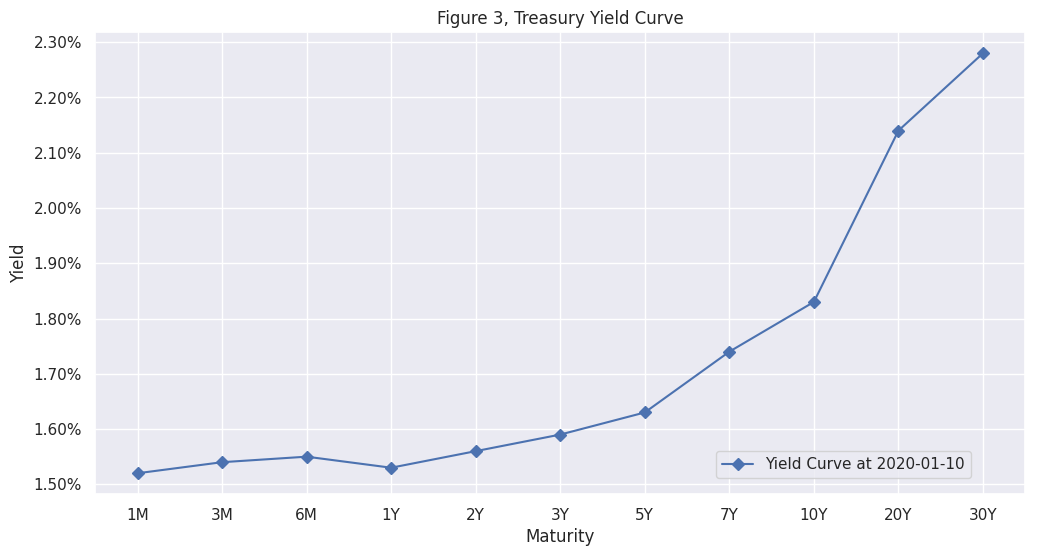
\includegraphics[width=0.8\textwidth]{gfx/m1l3_notes_fig3_yield_curve_2020-01-10.png}
    \caption{Hình 3, Đường cong Lợi suất Trái phiếu Kho bạc}
    \label{fig:m1l3_fig3}
\end{figure}

Trong phần này, chúng ta sẽ sử dụng kỹ thuật khớp đa thức (polynomial fitting) để ước tính một đường cong lợi suất.

Khớp đa thức là khi một nhà nghiên cứu sử dụng các đa thức bậc $n$ của biến đầu vào để dự đoán biến đầu ra. Ví dụ, nếu biến đầu vào là $x$ và biến đầu ra là $y$, biểu thức sau đây sẽ sử dụng các đa thức bậc $n$ của $x$ để dự đoán $y$.

$$y=\beta_{0}+\beta_{1}x_{1}+\beta_{2}x^{2}+\beta_{3}x^{3}...+\beta_{n}x^{n}$$

$\beta_{0},\beta_{1},\beta_{2},\beta_{3},...,\beta_{n}$ là các tham số cần được ước tính.
Có một số phương pháp khớp đa thức để khớp một đường cong lợi suất. Trong bài học này, chúng ta sẽ học hai phương pháp: mô hình Nelson Siegel và khớp spline bậc ba.

\subsection[Mô hình Nelson Siegel]{Mô hình Nelson Siegel (Nelson Siegel Model)}

Mô hình Nelson Siegel (mô hình NS) là một mô hình phổ biến để mô tả mối quan hệ giữa kỳ hạn và lợi suất (Svensson). Dưới đây là công thức của mô hình:

$$y(t)=\beta_{0}+\beta_{1}\left(\frac{1-e^{-\lambda t}}{\lambda t}\right)+\beta_{2}\left(\frac{1-e^{-\lambda t}}{\lambda t}-e^{-\lambda t}\right)+\epsilon$$

$\beta_{0},\beta_{1},\beta_{2}$ là các tham số cần được ước tính. $t$ là thời gian đáo hạn và $\lambda$ là tốc độ phân rã (decay rate). Tốc độ phân rã nằm trong khoảng từ 0 đến 1.
$\beta_{0}$ được dùng để mô tả mức độ (level) của đường cong lợi suất. $\beta_{1}$ được dùng để mô tả độ dốc (slope) của đường cong lợi suất và $\beta_{2}$ được dùng để mô tả hình dạng (shape) của đường cong lợi suất. Vì lý do này, chúng ta cũng gọi mô hình NS là mô hình nhân tố đường cong lợi suất.
Mô hình NS phân tách đường cong lợi suất thành ba phần tử như mô tả ở trên.
Tốc độ phân rã hoạt động như thế nào? Tốc độ phân rã càng nhỏ, đường cong phân rã càng chậm. Tốc độ phân rã càng lớn, đường cong phân rã càng nhanh. Tốc độ phân rã cho thấy lợi suất sẽ hội tụ nhanh đến mức nào về mức trung bình dài hạn.

Với cấu trúc đơn giản của mô hình NS, chúng ta có thể sử dụng các phần tử khác nhau trong mô hình để mô tả các hành vi khác nhau của đường cong lợi suất. Một khi chúng ta có được một ước lượng mô hình NS, chúng ta có thể sử dụng mô hình này để dự đoán diễn biến của những thay đổi lãi suất trong tương lai (Pape).

Hãy sử dụng gói Nelson Siegel Sevensson từ Python để chứng minh mô hình NS.

\subsection[Mô hình Nelson Siegel: Ứng dụng Python]{Mô hình Nelson Siegel: Ứng dụng Python (Nelson Siegel Model: Python Demonstration)}

Trong phần này, chúng ta sẽ sử dụng gói Nelson Siegel Sevensson từ Python để chỉ ra cách khớp một đường cong lợi suất. Đầu tiên, chúng ta cần cài đặt và import gói này.

\begin{lstlisting}[language=Python]
In [7]: pip install nelson_siegel_svensson
\end{lstlisting}

\begin{lstlisting}[language=Python]
Collecting nelson_siegel_svensson
  Downloading nelson_siegel_svensson-0.5.0-py2.py3-none-any.whl.metadata (6.
7 kB)
Collecting Click>=8.0 (from nelson_siegel_svensson)
  Downloading click-8.3.1-py3-none-any.whl.metadata (2.6 kB)
Requirement already satisfied: numpy>=1.22 in /usr/local/lib/python3.11/site
-packages (from nelson_siegel_svensson) (2.1.3)
...
Installing collected packages: Click, nelson_siegel_svensson
Successfully installed Click-8.3.1 nelson_siegel_svensson-0.5.0
WARNING: Running pip as the 'root' user can result in broken permissions and
conflicting behaviour with the system package manager, possibly rendering yo
ur system unusable. It is recommended to use a virtual environment instead:
https://pip.pypa.io/warnings/venv. Use the root-user-action option if you
know what you are doing and want to suppress this warning.
[notice] A new release of pip is available: 25.0.1 -> 25.3
[notice] To update, run: pip install --upgrade pip
Note: you may need to restart the kernel to use updated packages.
\end{lstlisting}

\begin{lstlisting}[language=Python]
In [8]: # Import the packages for fitting NS model
        from nelson_siegel_svensson.calibrate import calibrate_ns_ols
        import numpy as np
\end{lstlisting}

Sau khi import các gói cần thiết để khớp mô hình NS, chúng ta cần tạo các biến số cho việc lập mô hình. Đầu tiên chúng ta cần tạo một biến số kỳ hạn $t$ theo đơn vị năm. Ví dụ, 1 tháng là 0.08333 năm và 3 tháng là 0.25 năm. Biến số tiếp theo là biến số lợi suất. Cả biến kỳ hạn và biến lợi suất cần phải ở dưới dạng mảng (array form). Chúng ta sẽ sử dụng lợi suất từ ngày 10 tháng 1 năm 2020 (2020-01-10) làm ví dụ vì chúng ta vừa vẽ biểu đồ đường cong lợi suất vào ngày đó ở phần trước.

\begin{lstlisting}[language=Python]
In [9]: # Create maturity and yield variables in array form
        t = np.array([0.08333,0.25,0.5,1,2,3,5,7,10,20,30])
        y = np.array(yields.loc["2020-01-10"])
\end{lstlisting}

Sau khi các biến đã sẵn sàng, chúng ta có thể chuyển sang ước tính mô hình NS.

\begin{lstlisting}[language=Python]
In [10]: # Fit an NS model for yields from 2020-01-10
         curve, status = calibrate_ns_ols(t, y, tau0=1.0) # starting value of 1.0 fc
         assert status.success
         print(curve)
\end{lstlisting}

\begin{lstlisting}[language=Python]
NelsonSiegelCurve(beta0=np.float64(2.637682060451667), beta1=np.float64(-1.1
025872497097822), beta2=np.float64(-1.140646506802234), tau=np.float64(4.750
029828985478))
\end{lstlisting}

Kết quả của mô hình NS hiển thị $\beta_{0}$, $\beta_{1}$, $\beta_{2}$, và tốc độ phân rã đã được ước lượng. Bây giờ chúng ta hãy vẽ đồ thị để hiểu rõ hơn về kết quả mô hình.

\begin{lstlisting}[language=Python]
In [11]: y_hat = curve
         t_hat = np.linspace(0.5,30,100)
         plt.plot(t_hat, y_hat(t_hat))
         plt.xlabel("Maturity")
         plt.ylabel("Yield")
         plt.title("Figure 4, NS Model Result")
\end{lstlisting}

\begin{lstlisting}[language=Python]
Out [11]: Text(0.5, 1.0, 'Figure 4, NS Model Result')
\end{lstlisting}

\begin{figure}[htbp]
    \centering
    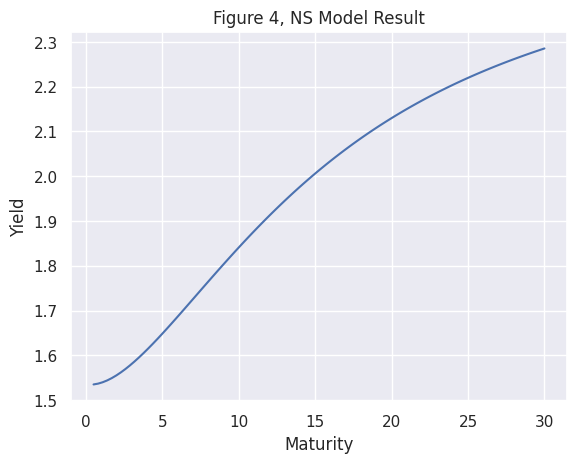
\includegraphics[width=0.8\textwidth]{gfx/m1l3_notes_fig4_ns_model_result.png}
    \caption{Hình 4, Kết quả Mô hình NS}
    \label{fig:m1l3_fig4}
\end{figure}

Từ Hình 4 ở trên, chúng ta có thể thấy đường cong lợi suất được ước tính khá khớp với biểu đồ đường cong mà chúng ta đã vẽ ở phần trước. Hãy thử ước tính một hình dạng khác của đường cong lợi suất. Lần này, chúng ta sẽ sử dụng lợi suất từ ngày 23 tháng 3 năm 2006 (2006-03-23). Trước tiên, hãy vẽ dữ liệu lợi suất từ 2006-03-23.

\begin{lstlisting}[language=Python]
In [12]: plot_yield_curve('2006-03-23', 'Figure 5, ')
\end{lstlisting}

\begin{lstlisting}[language=Python]
/tmp/ipykernel_18/1226209266.py:6: UserWarning: set_ticklabels() should only
be used with a fixed number of ticks, i.e. after set_ticks() or using a Fixe
dLocator.
  ax.set_yticklabels(['{:.2f}%'.format(y) for y in ax.get_yticks()])
\end{lstlisting}

\begin{figure}[htbp]
    \centering
    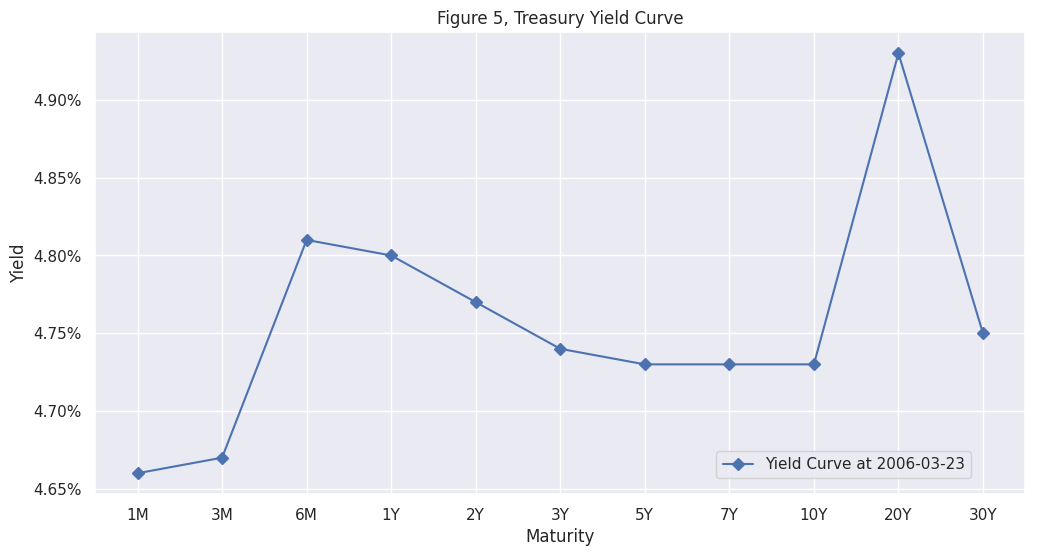
\includegraphics[width=0.8\textwidth]{gfx/m1l3_notes_fig5_yield_curve_2006-03-23.png}
    \caption{Hình 5, Đường cong Lợi suất Trái phiếu Kho bạc}
    \label{fig:m1l3_fig5}
\end{figure}

Trong Hình 5, các mức lợi suất từ kỳ hạn 6 tháng đến kỳ hạn 10 năm thể hiện hình dạng dốc xuống, điều này khác với đường cong lợi suất vào ngày 2020-01-10. Hãy xem liệu mô hình NS có nhận ra điều này hay không. Chúng ta sẽ lặp lại cùng quy trình đó để mô hình hóa đường cong lợi suất vào ngày 2006-03-23.

\begin{lstlisting}[language=Python]
In [13]: y = np.array(yields.loc["2006-03-23"])
         curve, status = calibrate_ns_ols(t, y, tau0=0.5) # starting value of 0.5 fo
         assert status.success
         print(curve)
\end{lstlisting}

\begin{lstlisting}[language=Python]
NelsonSiegelCurve(beta0=np.float64(4.7693015468990705), beta1=np.float64(-0.
1860856799305238), beta2=np.float64(0.25937117013919064), tau=np.float64(0.2
5704895433346897))
\end{lstlisting}

\begin{lstlisting}[language=Python]
In [14]: y_hat = curve
         t_hat = np.linspace(0.5,30,100)
         plt.plot(t_hat, y_hat(t_hat))
         plt.xlabel("Maturity")
         plt.ylabel("Yield")
         plt.title("Figure 6, NS Model Result")
\end{lstlisting}

\begin{lstlisting}[language=Python]
Out [14]: Text(0.5, 1.0, 'Figure 6, NS Model Result')
\end{lstlisting}

\begin{figure}[htbp]
    \centering
    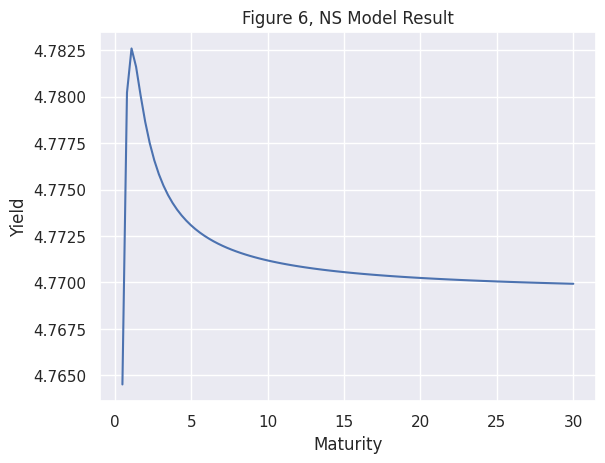
\includegraphics[width=0.8\textwidth]{gfx/m1l3_notes_fig6_ns_model_result2.png}
    \caption{Hình 6, Kết quả Mô hình NS}
    \label{fig:m1l3_fig6}
\end{figure}

Từ Hình 6 ở trên, chúng ta có thể thấy rằng đường cong dốc xuống sau một năm đáo hạn. Kết quả này nhất quán với Hình 5 mà chúng ta đã vẽ trước đó.

\section[Khớp Spline Bậc ba cho Đường cong Lợi suất]{Khớp Spline Bậc ba cho Đường cong Lợi suất (Cubic Spline Fitting of Yield Curve)}

Trong phần này, chúng ta sẽ giới thiệu một phương pháp phổ biến khác để khớp đường cong lợi suất với dữ liệu. Nó được gọi là spline bậc ba (cubic spline). Khớp spline là một phương pháp thuộc kỹ thuật khớp đa thức. Vui lòng đọc tài liệu bắt buộc "Phương pháp Nội suy Spline" để học lý thuyết về khớp spline, đặc biệt là khớp spline bậc ba. Chúng ta sẽ sử dụng phương pháp khớp spline bậc ba trong Python để khớp một đường cong lợi suất trong phần tiếp theo. Xin lưu ý rằng trong Bài 4 "Ứng dụng của Nội suy Spline Bậc hai", có một sai sót trong phần ghi chú. Trong ma trận lớn được trình bày, vector hệ số đáng lẽ phải nằm ở phía bên trái của phương trình, không phải ở phía bên phải.

\subsection[Ứng dụng Python: Sử dụng Khớp Spline Bậc ba để Khớp một Đường cong Lợi suất]{Ứng dụng Python: Sử dụng Khớp Spline Bậc ba để Khớp một Đường cong Lợi suất (Python Application: Use Cubic Spline Fitting to Fit a Yield Curve)}

Trong phần này, chúng ta sẽ chứng minh cách khớp một đường cong lợi suất bằng spline bậc ba. Để thuận tiện cho việc minh họa, chúng ta sẽ chỉ sử dụng lợi suất từ các Trái phiếu Kho bạc kỳ hạn 2 năm, 5 năm, 10 năm và 30 năm vào ngày 2020-01-10 làm ví dụ. Đầu tiên, hãy kiểm tra các lợi suất vào ngày 2020-01-10.

\begin{lstlisting}[language=Python]
In [15]: yields.loc["2020-01-10"]
\end{lstlisting}

\begin{lstlisting}[language=Python]
Out [15]: 1 Month     1.52
          3 Month     1.54
          6 Month     1.55
          1 Year      1.53
          2 Year      1.56
          3 Year      1.59
          5 Year      1.63
          7 Year      1.74
          10 Year     1.83
          20 Year     2.14
          30 Year     2.28
          Name: 2020-01-10 00:00:00, dtype: float64
\end{lstlisting}

Hãy định nghĩa biến số kỳ hạn và biến số lợi suất dưới dạng các mảng.

\begin{lstlisting}[language=Python]
In [16]: t = np.array([2,5,10,30])
         y = np.array([1.56,1.63,1.83,2.28])
\end{lstlisting}

Bây giờ, chúng ta hãy viết ra các phương trình spline bậc ba trước. Vì chúng ta có 4 điểm dữ liệu theo cặp, nên sẽ có 3 hàm spline.

$$f(x)=a_{1}x^{3}+b_{1}x^{2}+c_{1}x+d_{1}, \text{ khi } 2\le x\le 5$$
$$f(x)=a_{2}x^{3}+b_{2}x^{2}+c_{2}x+d_{2}, \text{ khi } 5\le x\le 10$$
$$f(x)=a_{3}x^{3}+b_{3}x^{2}+c_{3}x+d_{3}, \text{ khi } 10\le x\le 30$$

Từ các phương trình trên, chúng ta có 12 ẩn số. Do đó, chúng ta cần 12 phương trình để giải cho 12 tham số. Hãy viết ra các phương trình mà mỗi hàm spline bậc ba sẽ đi qua tại hai điểm dữ liệu liên tiếp.

$$a_{1}(2)^{3}+b_{1}(2)^{2}+c_{1}(2)+d_{1}=1.56\;\;\;(1)$$
$$a_{1}(5)^{3}+b_{1}(5)^{2}+c_{1}(5)+d_{1}=1.63\;\;\;(2)$$
$$a_{2}(5)^{3}+b_{2}(5)^{2}+c_{2}(5)+d_{2}=1.63\;\;\;(3)$$
$$a_{2}(10)^{3}+b_{2}(10)^{2}+c_{2}(10)+d_{2}=1.83\;\;\;(4)$$
$$a_{3}(10)^{3}+b_{3}(10)^{2}+c_{3}(10)+d_{3}=1.83\;\;\;(5)$$
$$a_{3}(30)^{3}+b_{3}(30)^{2}+c_{3}(30)+d_{3}=2.28\;\;\;(6)$$

Bây giờ, hãy viết các phương trình cho thấy đạo hàm bậc nhất của hai hàm spline bậc ba liên tiếp là liên tục tại các điểm bên trong chung.

$$3a_{1}(5)^{2}+2b_{1}(5)+c_{1}=3a_{2}(5)^{2}+2b_{2}(5)+c_{2}\;\;\;(7)$$
$$3a_{2}(10)^{2}+2b_{2}(10)+c_{2}=3a_{3}(10)^{2}+2b_{3}(10)+c_{3}\;\;\;(8)$$

Và sau đó chúng ta sẽ viết các phương trình cho thấy đạo hàm bậc hai của hai hàm spline bậc ba liên tiếp là liên tục tại các điểm bên trong chung.

$$6a_{1}(5)+2b_{1}=6a_{2}(5)+2b_{2}\;\;\;(9)$$
$$6a_{2}(10)+2b_{2}=6a_{3}(10)+2b_{3}\;\;\;(10)$$

Hai phương trình cuối cùng là các điều kiện biên. Chúng ta đặt các đạo hàm bậc hai của các hàm spline bậc ba tại các điểm đầu mút bằng không.

$$6a_{1}(2)+2b_{1}=0\;\;\;(11)$$
$$6a_{3}(30)+2b_{3}=0\;\;\;(12)$$

Giờ chúng ta đã có 12 phương trình để giải cho 12 tham số. Chúng ta có thể viết toàn bộ bài toán này dưới dạng một phương trình ma trận lớn.

$$
\begin{bmatrix} 
8 & 4 & 2 & 1 & 0 & 0 & 0 & 0 & 0 & 0 & 0 & 0 \\ 
125 & 25 & 5 & 1 & 0 & 0 & 0 & 0 & 0 & 0 & 0 & 0 \\ 
0 & 0 & 0 & 0 & 125 & 25 & 5 & 1 & 0 & 0 & 0 & 0 \\ 
0 & 0 & 0 & 0 & 1000 & 100 & 10 & 1 & 0 & 0 & 0 & 0 \\ 
0 & 0 & 0 & 0 & 0 & 0 & 0 & 0 & 1000 & 100 & 10 & 1 \\ 
0 & 0 & 0 & 0 & 0 & 0 & 0 & 0 & 27000 & 900 & 30 & 1 \\ 
75 & 10 & 1 & 0 & -75 & -10 & -1 & 0 & 0 & 0 & 0 & 0 \\ 
0 & 0 & 0 & 0 & 300 & 20 & 1 & 0 & -300 & -20 & -1 & 0 \\ 
30 & 2 & 0 & 0 & -30 & 2 & 0 & 0 & 0 & 0 & 0 & 0 \\ 
0 & 0 & 0 & 0 & 60 & 2 & 0 & 0 & -60 & -2 & 0 & 0 \\ 
12 & 2 & 0 & 0 & 0 & 0 & 0 & 0 & 0 & 0 & 0 & 0 \\ 
0 & 0 & 0 & 0 & 0 & 0 & 0 & 0 & 180 & 2 & 0 & 0 
\end{bmatrix}
\bullet
\begin{bmatrix} 
a_{1} \\ b_{1} \\ c_{1} \\ d_{1} \\ a_{2} \\ b_{2} \\ c_{2} \\ d_{2} \\ a_{3} \\ b_{3} \\ c_{3} \\ d_{3}
\end{bmatrix}
=
\begin{bmatrix} 
1.56 \\ 1.63 \\ 1.63 \\ 1.83 \\ 1.83 \\ 2.28 \\ 0 \\ 0 \\ 0 \\ 0 \\ 0 \\ 0 
\end{bmatrix}
$$

Chúng ta có thể viết phương trình ma trận trên dưới dạng phương trình sau:

$$A\bullet c=y$$

$A$ là ma trận vuông. $c$ là vector hệ số và $y$ là vector đầu ra. Để giải cho $c$, chúng ta sẽ sử dụng quy tắc đại số tuyến tính sau đây.

$$c=A^{-1}\bullet y$$

$A^{-1}$ là ma trận nghịch đảo của ma trận vuông. Đoạn mã Python sau được dùng để giải tìm vector hệ số.

\begin{lstlisting}[language=Python]
In [17]: # Create output vector y (out variable) and squared matrix A (input variable
         out = np.array([1.56,1.63,1.63,1.83,1.83,2.28,0,0,0,0,0,0])
         input = np.array([[8,4,2,1,0,0,0,0,0,0,0,0], [125,25,5,1,0,0,0,0,0,0,0,0], [0,
         [0,0,0,0,0,0,0,0,1000,100,10,1], [0,0,0,0,0,0,0,0,27000,900
         [30,2,0,0,-30,-2,0,0,0,0,0,0], [0,0,0,0,60,2,0,0,-60,-2,0,0
\end{lstlisting}

\begin{lstlisting}[language=Python]
In [18]: # Solve for coefficient vector and reshape to an 3 by 4 array (lines variabl
         # Make sure to give enough decimals since all coefficients are relatively sm
         lines = np.round(np.dot(np.linalg.inv(input), out).reshape(-1,4), decimals=8)
         lines
\end{lstlisting}

\begin{lstlisting}[language=Python]
Out [18]: array([[ 3.96060000e-04, -2.37634000e-03,  2.45215100e-02,
                   1.51729391e+00],
                 [-3.31400000e-04,  8.53548000e-03, -3.00376300e-02,
                   1.60822581e+00],
                 [ 2.34400000e-05, -2.10968000e-03,  7.64139800e-02,
                   1.25338710e+00]])
\end{lstlisting}

Từ kết quả trên, chúng ta có thể thấy các hệ số được trình bày dưới dạng một mảng $3\times4$.

$$
\begin{bmatrix} a_{1} & b_{1} & c_{1} & d_{1} \\ a_{2} & b_{2} & c_{2} & d_{2} \\ a_{3} & b_{3} & c_{3} & d_{3} \end{bmatrix}
$$

Bây giờ chúng ta có thể vẽ một đường cong mượt mà từ kỳ hạn 2 đến kỳ hạn 30 bằng Python.

\begin{lstlisting}[language=Python]
In [16]: # Calculates x**0 + x**1 + x**2 + x**3
         def plot_num(values, coeffs):
             # Coeffs are assumed to be in order 0, 1, ..., n-1
             expanded = np.hstack([coeffs[i] * (values ** i) for i in range(0, len(cc
             return np.sum(expanded, axis=1)
\end{lstlisting}

\begin{lstlisting}[language=Python]
In [17]: # Simulate the 100 paired data points and draw the graph
         xs = np.linspace(2,30, 100)
         y1s = plot_num(xs[xs<5].reshape(-1,1), lines[0][::-1])
         y2s = plot_num(xs[(xs>=5) & (xs<10)].reshape(-1,1), lines[1][::-1])
         y3s = plot_num(xs[xs>=10].reshape(-1,1), lines[2][::-1])
         ys = np.concatenate([y1s, y2s, y3s])
         
         plt.plot(xs, ys)
         plt.scatter(t, y,c="red")
         plt.xlabel("Maturity")
         plt.ylabel("Yield")
         plt.title("Figure 7")
         plt.show()
\end{lstlisting}

\begin{figure}[htbp]
    \centering
    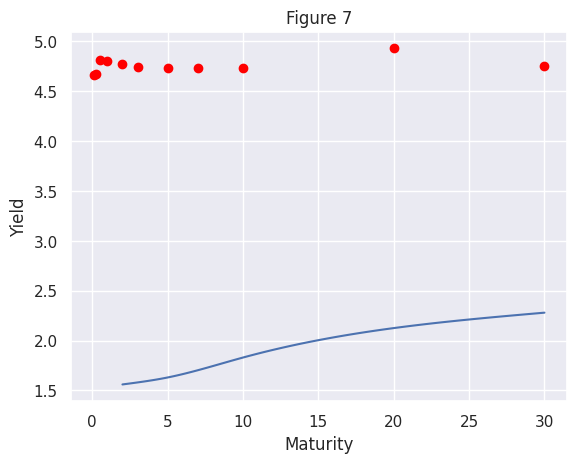
\includegraphics[width=0.8\textwidth]{gfx/m1l3_notes_fig7_cubic_spline_fit.png}
    \caption{Hình 7}
    \label{fig:m1l3_fig7}
\end{figure}

Hình 7 ở trên thể hiện đường cong lợi suất ước tính vào ngày 2020-01-10 bằng cách sử dụng phương pháp khớp spline bậc ba. Chúng ta có thể thấy với spline bậc ba, đường nối giữa hai điểm dữ liệu không phải là đường thẳng mà là đường cong. Với đường cong ước lượng này, chúng ta có thể tính toán lợi suất cho bất kỳ kỳ hạn nào nằm trên đường cong này nhằm mục đích định giá trái phiếu hoặc các phân tích lợi suất khác. Một khi chúng ta đã xây dựng được đường cong lợi suất này, chúng ta có thể dùng nó để lấy hệ số chiết khấu cho bất kỳ dòng tiền nào trong tương lai. Bằng cách tính tổng tất cả các dòng tiền trong tương lai đã chiết khấu từ một tài sản, chúng ta có thể có được giá trị hiện tại của tài sản đó và đánh giá xem liệu giá trị hiện tại đang định giá cao hay thấp hơn so với giá trị thực của tài sản.

\section[Kết luận]{Kết luận (Conclusion)}

Trong bài học này, đầu tiên chúng ta đã học xem lãi suất phi rủi ro là gì. Sau đó, chúng ta tính toán độ biến động của trái phiếu Kho bạc Hoa Kỳ tại các kỳ hạn khác nhau. Chúng ta cũng đã học hai phương pháp để khớp đường cong lợi suất bằng phương pháp Nelson Siegel và phương pháp spline bậc ba. Cuối cùng, chúng ta đã chứng minh cách triển khai hai phương pháp này để khớp đường cong lợi suất Trái phiếu Kho bạc Hoa Kỳ trong Python.

\section*{Tài liệu tham khảo (References)}

\begin{itemize}
    \item Pape. "Understanding the Nelson-Siegel-Svensson (NSS) Model for Bond Yield Curve Analysis." Medium, 2024 May 12. \url{https://medium.com/@pape14/understanding-the-nelson-siegel-svensson-nss-model-for-bond-yield-curve-analysis-2a23202cbf6b}.
    \item Svensson, Lars. "Estimating and Interpreting Forward Interest Rates: Sweden 1992-1994." NBER Working Paper Series, no. 4871, 1994.
\end{itemize}

Copyright 2024 WorldQuant University. This content is licensed solely for personal use. Redistribution or publication of this material is strictly prohibited.

